\section{Problem A}
    \subsection{Statement}
        Given a graph and a spanning tree of the graph, determine whether the spanning tree is a valid BFS
        tree of the graph (rooted at $1$).

    \subsection{Solution}
        First, an obvious necessary condition is that the distances of each vertex should be the same in the graph
        and the tree.

        Rather lazily, we ask ``Is this condition also sufficient?''.

        Let's see for example the graph $G$ with the vertex set
        $V = \left\{1, 2, 3, 4, 5\right\}$ and the edge set 
        $E = \left\{12, 13, 24, 25, 35\right\}$.

        And consider the spanning tree $T$ with the edge set
        $E' = \left\{12, 13, 24, 35\right\}$, so the parents
        of $4$ and $5$ are $2$ and $3$ respectively.

        \begin{figure}[h]
        \centering
        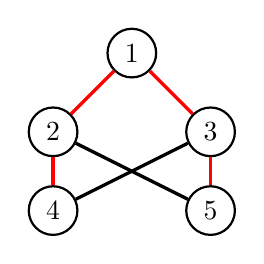
\begin{tikzpicture}
        \begin{scope}[every node/.style={circle, thick, draw}]
            \node (v1) at (2.5, 4) {1};
            \node (v2) at (1.5, 3) {2};
            \node (v3) at (3.5, 3) {3};
            \node (v4) at (1.5, 2) {4};
            \node (v5) at (3.5, 2) {5};
        \end{scope}

        \begin{scope}[
            every edge/.style={draw=red,very thick}]
            \path [-] (v1) edge (v2);
            \path [-] (v1) edge (v3);
            \path [-] (v2) edge (v4);
            \path [-] (v3) edge (v5);
            
        \end{scope}

        \begin{scope}[
            every edge/.style={draw=black,very thick}]
            \path [-] (v2) edge (v5);
            \path [-] (v3) edge (v4);

        \end{scope}
        \end{tikzpicture}
        \caption{The graph $G$, with the edges of $T$ in red} \label{fig:naive}
        \end{figure}

        By examining the figure, you can see that $T$ is not a BFS-tree, so the obvious necessary
        condition is not sufficient $\ddot\smallfrown$

        But having verified the obvious condition, it turns out we only need one more insight
        to get a polynomial time solution.
        (pause here if you want to try to find it yourself)

        Denote by $p(v)$ the parent of $v$ in the spanning tree,
        and by $d(v)$ the distance of $v$ from $1$ in the spanning tree
        (and the graph).

        Then we require that for all $v$, $p(v)$ is ``explored''
        in the BFS before all such $u$ in the graph such that
        $d(u) + 1 = d(v)$, and the edge $uv$ is in the graph $G$,
        and $u \neq p(v)$.
        For brevity, define the set
        $U = \left\{u \mid u \in V\setminus \left\{p(v)\right\}, d(u) + 1 = d(v), uv \in E\right\}$,
        and denote by $p^k(v)$ the $k^{\texttt{th}}$ ancestor of $v$.

        ``Explored'' is, of course, equivalent to being popped from the BFS
        queue, which happens in the same order as insertion, so we
        need $p(v)$ to be inserted before all $u \in U$.
        How can we ensure that? We have to push $p(p(v))$ before
        $p(u)$ for all $u \in U$. And this effect cascades, until the
        least common ancestor of $p(v)$ and $u$ in the tree $T$.

        In general, for all $u \in U$, we need to explore
        $p^k(v)$ before $p^{k - 1}(u)$ when
        $p^k(v) \neq p^{k - 1}(u)$.

        We can represent this requirement in an auxilary di-graph
        $G'$ with the same vertex set as $G$,
        with a directed edge from $x \to y$ denoting that
        $x$ needs to be explored before $y$.

        \begin{figure}[h]
        \centering
        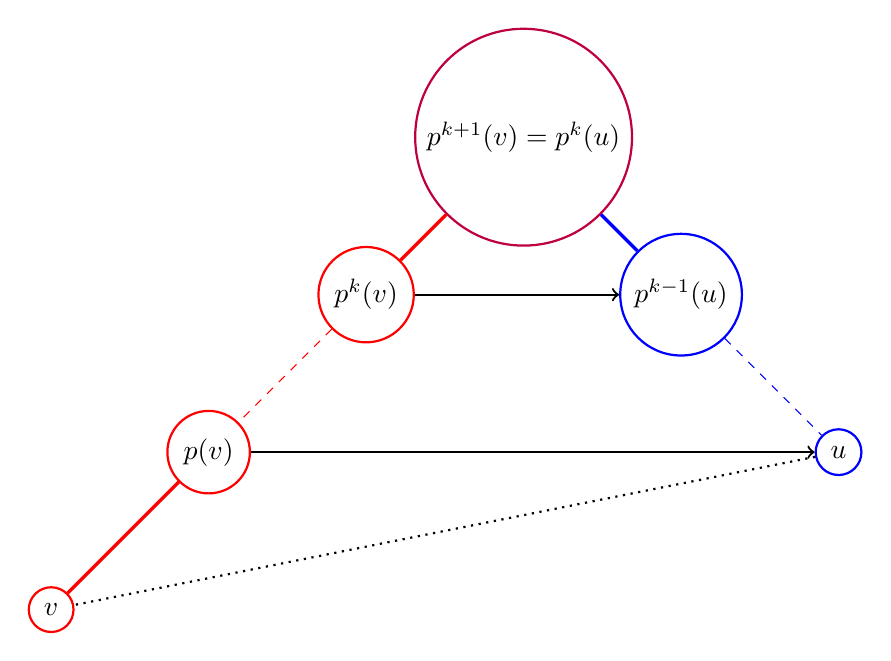
\begin{tikzpicture}
        \begin{scope}[
            tnode/.style={draw=red, circle, thick},
            gnode/.style={draw=blue, circle, thick},
            mnode/.style={draw=purple, circle, thick}]
            \node[mnode] (lca) at (10, 10) {$p^{k+1}(v) = p^k(u)$};
            \node[tnode] (vk) at (8, 8) {$p^k(v)$};
            \node[tnode] (v1) at (6, 6) {$p(v)$};
            \node[tnode] (v) at (4, 4)  {$v$};
            \node[gnode] (u) at (14, 6)  {$u$};
            \node[gnode] (uk) at (12, 8) {$p^{k - 1}(u)$};
        \end{scope}

        \begin{scope}[
            every edge/.style={draw=red,very thick}]
            \path [-] (lca) edge (vk);
            \path [-] (v1) edge (v);
        \end{scope}

        \begin{scope}[
            every edge/.style={draw=blue,very thick}]
            \path [-] (lca) edge (uk);
        \end{scope}

        \begin{scope}[
            every edge/.style={draw=black,thick}]
            \path [->] (vk) edge (uk);
            \path [->] (v1) edge (u);
        \end{scope}

        \draw[dashed, red] (vk) -- (v1);
        \draw[dashed, blue] (uk) -- (u);
        \draw[dotted, thick] (u) -- (v);

        \end{tikzpicture}
        \caption{The dotted black line denotes the annoying edge which is causing all the shenanigans.
                The solid black lines with arrows denote edges in $G'$.
        }
        \label{fig:fancy}
        \end{figure}

        Finally, $G'$ has a cycle $\iff$ $T$ is not a BFS-tree.

        Since $G'$ has $O(EN)$ edges in the worst case, we need $O(EN)$
        time and space to construct it.

        Looking at Figure 2, we can note that all the directed
        edges are unnecessary, except the one from $p^k(v) \to p^{k-1}(u)$
        (proof left as exercise $\ddot\smallsmile$), so we can now have
        only $O(E)$ edges in $G'$.
        To construct it efficiently, we need to
        \begin{itemize}
            \item find the LCA of two nodes quickly
            \item find the node just below the LCA quickly
        \end{itemize}

        A topcoder tutorial shows how to compute LCAs in $O(\log N)$ per query
        with $O(N \log N)$ pre-processing
        {\color{blue} \href{https://www.topcoder.com/community/data-science/data-science-tutorials/range-minimum-query-and-lowest-common-ancestor/#Another%20easy%20solution%20in%20O(N%20logN,%20O(logN)}{here}}.

        You can also use the same idea as in the article linked above to compute the $k^{\texttt{th}}$
        ancestor in $O(\log N)$ per query, which is sufficient to compute the second item.

        Hence we have an $O(|E| \log N)$ solution, which is sufficient to pass all tests.